62. \begin{figure}[ht!]
\center{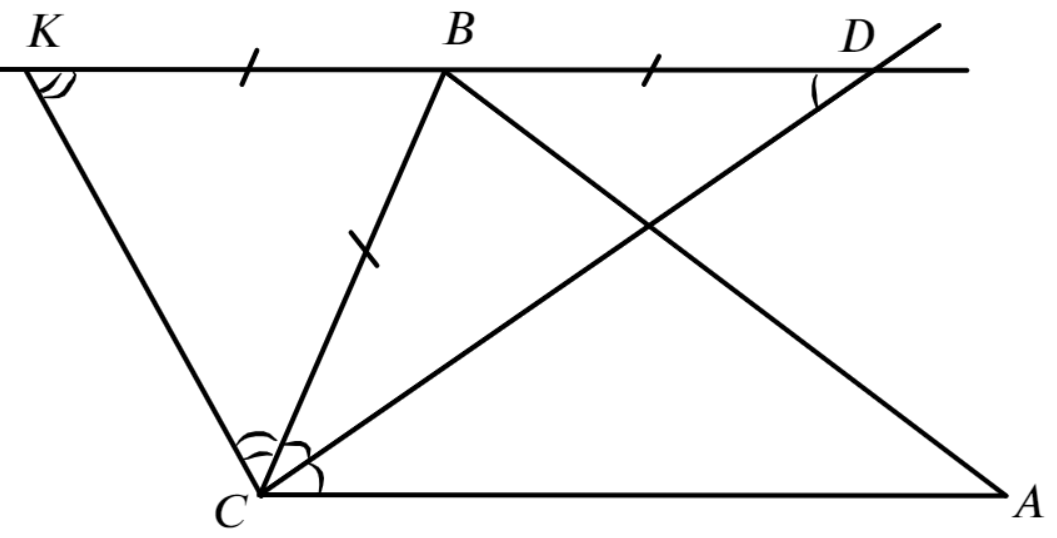
\includegraphics[scale=0.35]{g62.png}}
\end{figure}\\
Так как $KD\parallel AC,$ накрест лежащие углы $DCA$ и $BDC$ равны, а так как $CD$ является биссектрисой, $\angle BCD=\angle DCA=\angle BDC.$ Поэтому треугольник $BCD$ является равнобедренным и $BC=BD=KB,$ значит равнобедренным является и треугольник $KBC.$ Обозначим их углы при основании: $\angle BCD=x,\ \angle BCK=y.$ Тогда из треугольника $KCD$ имеем $2x+2y=180^\circ,\ x+y=90^\circ=\angle KCD,$ ч.т.д.
ewpage
oindent
